\documentclass{article} % For LaTeX2e
\usepackage{nips14submit_e,times}
\usepackage{hyperref}
\usepackage{url}
\usepackage{amsmath}
\usepackage{graphicx}
%\documentstyle[nips14submit_09,times,art10]{article} % For LaTeX 2.09


\title{Analysis of the Emergence of Echo Chambers in Social Networks: A simulative approach}


\author{
Varnan Dewangan \thanks{ https://github.com/awivawie/HSN619-project} \\
Department of Humanities and Social Sciences\\
IIT Roorkee\\
Uttarakhand, 247667 \\
\texttt{v\_dewangan@hs.iitr.ac.in}
}

% The \author macro works with any number of authors. There are two commands
% used to separate the names and addresses of multiple authors: \And and \AND.
%
% Using \And between authors leaves it to \LaTeX{} to determine where to break
% the lines. Using \AND forces a linebreak at that point. So, if \LaTeX{}
% puts 3 of 4 authors names on the first line, and the last on the second
% line, try using \AND instead of \And before the third author name.

\newcommand{\fix}{\marginpar{FIX}}
\newcommand{\new}{\marginpar{NEW}}

\nipsfinalcopy % Uncomment for camera-ready version

\begin{document}


\maketitle

\begin{abstract}
At this digital age, media is the primary channel for the exchange of information among the world. As these platforms provide direct access to an unprecedented amount of content to anyone from any where in the world. Recent studies have shown that users tend to select information adhering to their system of beliefs, and may cause the creation of "Echo Chambers" due to the phenomenon of homophily. This study examines echo chambers in social networks using a model that incorporates opinion dynamics and homophily-based rewiring. I simulated agents within a social network, where opinions evolve through interactions with neighbors, and agents rewire connections based on opinion similarity. The results show that this process fosters clustering of like-minded agents, demonstrating how homophily and opinion influence contribute to echo chamber formation. These findings illuminate mechanisms underlying polarized groups in social networks.
\end{abstract}



\section{Introduction}
\label{headings}
As online networks, such as social media, have developed
and increased in popularity, research regarding the spread of
false information, the polarization of opinions \cite{dandekar2013biased}, and create an echo-chamber phenomena. Social media may limit the exposure to diverse perspectives and favor the formation of groups of like-minded users framing and reinforcing a shared narrative, that is, echo chambers.\cite{cinelli2021echo}

Recently, questions regarding how individuals on a network receive new information and form or adopt opinions has come to the fore. Whether on topics of national referendum, deciding between presidential candidates, or interpreting news events, it has become more and more common for such information to be ascertained via social media. They reinforce biases and hinder information diversity. 

This study models echo chamber formation by simulating a network of agents whose opinions evolve and connections rewire based on homophily. Homophily - our tendency to surround ourselves with others who share our perspectives and opinions about the world - is both a part of human nature and an organizing principle underpinning many of our digital social networks.\cite{gillani2018me} We aim to understand the extent to which different initialization schemes and rewiring rules affect opinion convergence and network structure. Our goal is to understand how opinion dynamics and homophily-driven rewiring jointly contribute to clustering of opinions using an agent based network.

\section{Model and Methodology}
The models involve a network of agents initialized with opinions. The agents update their opinions and connections based on homophily. Both models are implemented in Python using \texttt{numpy}, \texttt{networkx}, and \texttt{matplotlib} for efficient computation, graph manipulation, and visualization.

\subsection{Network and Agent Initialization}
In both methods, we create a random network with a specified number of agents and links.

Both models feature an \texttt{Agent} class representing individuals in the network, each initialized with an opinion. The \texttt{Agent} class contains few components. Firstly 
Attributes,  each \texttt{Agent} is assigned an \texttt{id} and an initial \texttt{opinion}. The opinion reflects the agent’s perspective, which can range between -1 (opposing) and +1 (supporting) in the model. Here, opinion dynamics are driven by either the \textbf{Opinion Updates} where Agents align their opinions closer to similar neighbors. and contains \textbf{Rewiring Mechanisms} where agents adjust connections based on homophily, reinforcing links with similar agents while breaking ties with dissimilar ones.

In our study, we employed two models to simulate the formation of echo chambers in social networks, each using a homophily-based rewiring mechanism. This section outlines methodology and functionality while explaining how opinions and connections evolve over time to foster network polarization.

\subsection{Echo Chamber Model (Network Initialization and Opinion Update)}
The \texttt{EchoChamberModel} class manages the network, encompassing all agents and their connections. In both models, this class is initialized with parameters that define the network structure and behavior:
\begin{itemize}
    \item \textbf{Number of Agents (\texttt{num\_agents})}: Defines the size of the network, which influences how interactions scale.
    \item \textbf{Initial Links (\texttt{initial\_links})}: Specifies the number of edges (connections) in the random network. Initial links are established randomly, allowing agents to have diverse connections at the start.
    \item \textbf{Homophily Factor (\texttt{homophily\_factor})}: Determines the threshold of opinion similarity required for agents to maintain or form links.  This factor is an important aspect of the echo chamber simulation, which translates to greater aspect of similarity of the opinions, because it controls the agent's decision on whose opinions are close enough to influence their own. A lower homplily factor will increase the selectivity of the agents, this setting will lead to stronger clustering and slower opinion shifts. Conversely, higher homophily factor will increase the flexibility of acceptance of varied opinions by the agents. This can dilute strong opinion clusters and create a more homogenous network.

\end{itemize}

In both models, the network is initialized as a directed random graph using NetworkX’s \texttt{gnm\_random\_graph} function, creating a basic network where agents are randomly connected. 

Opinions are initialized with random values uniformly distributed between -1 and 1. This approach introduces a broader range of opinions from the beginning, resulting in a more gradual clustering process as agents gravitate towards various opinion “poles” .Once initialized, each agent’s opinion is stored as an attribute within the network nodes, allowing the model to track opinion changes at both the agent and network levels.

\subsubsection{Opinion Update Process}
Each agent adjusts their opinion based on the opinions of their neighbors. Neighbors are considered similar if their opinions differ from a node's opinion by less than a defined threshold. This mechanism adjusts the agent's opinion based on the average opinion of its similar neighbors, gradually aligning it towards the consensus within its immediate social circle. 

\begin{equation}
 O_{i}^{t+1} = O_{i}^{t} + 0.1 \times (\text{mean}(O_{\text{similar neighbors}}) - O_{i}^{t})
\end{equation}

During each simulation step, agents update their opinions based on interactions with their neighbors. The model iterates over each agent’s neighbors to identify those whose opinions are sufficiently similar (i.e., within the homophily threshold). If similar neighbors exist, the agent’s opinion shifts slightly towards the average opinion of these neighbors, reinforcing clustering and aiding in the emergence of echo chambers.

\subsubsection{Rewiring Mechanism}
In addition to opinion updates, agents in both models periodically rewire their network connections based on homophily. 
the Homophily threshold reflects an agent’s preference for disconnecting from neighbors who hold significantly different views. This threshold enforces that only sufficiently similar agents remain connected over time.The process further reinforces clustering and the emergence of echo chambers.

\begin{equation}
\text{Rewire\:if}\quad |O_i - O_j| \geq \text{threshold\:(homophily\:factor)}
\end{equation}

At each simulation step, the model randomly selects agents for potential rewiring with a set probability (10\%). 

\subsection{Model Execution and Analysis}
To simulate opinion dynamics and measure the resulting echo chambers, each model runs through a sequence of steps, updating opinions and rewiring connections at each iteration. The models include several analysis metrics and visualizations that allow us to observe how clustering unfolds over time. The initial value of parameters is shown in the Table \ref{sample-table}.

\begin{figure}[h]
    \centering
    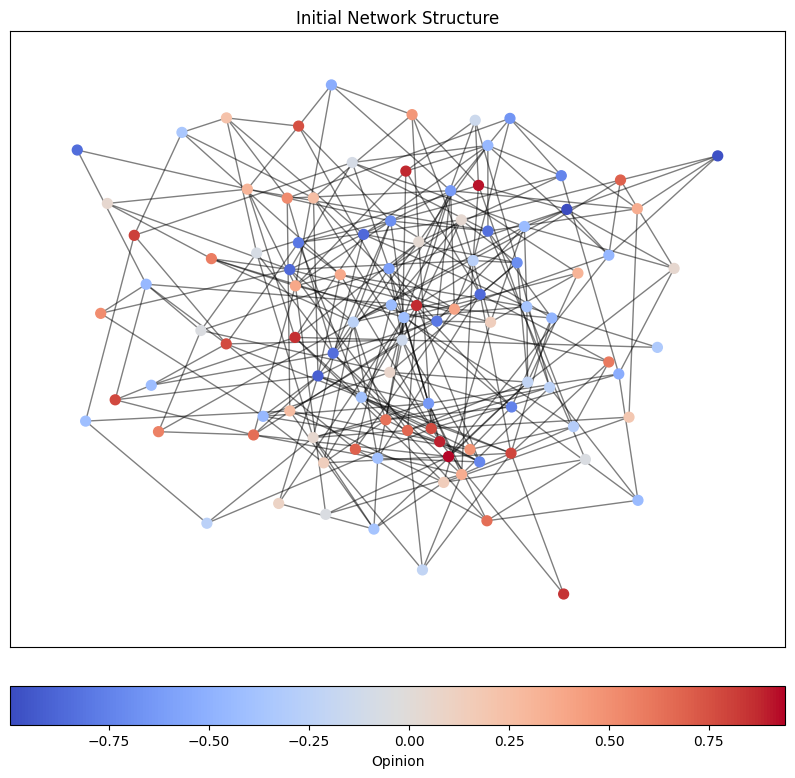
\includegraphics[width=0.7\linewidth]{download-2.png}
    \caption{Initial visualization of network with continuous opinion variable}
    \label{fig:c1}
\end{figure}

\begin{figure}
    \centering
    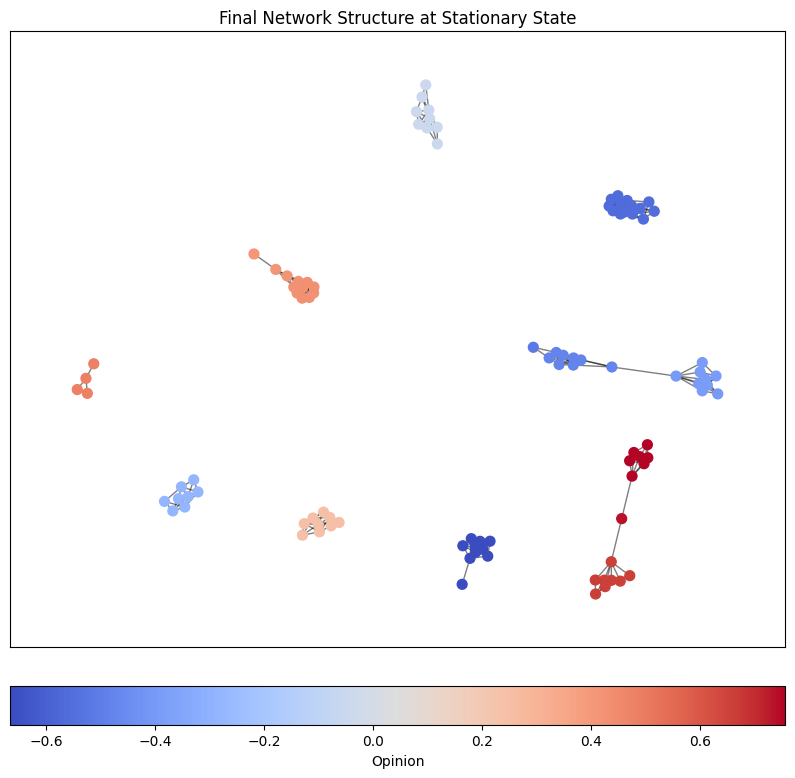
\includegraphics[width=0.7\linewidth]{download-1.png}
    \caption{Final visualization of Network with continuous opinion variable, at stationary state}
    \label{fig:c2}
\end{figure}


The initial and final network structures provide a visual representation of the clustering process of both the binary and continuous variable initializations
\textbf{Initial Network} is similar with varied opinions for both versions,It is a Randomly connected network with no distinct clusters as shown in Figure  \ref{fig:c1} .
The \textbf{Final Network}  converges into multiple clusters, indicating strong polarization. The clusters on figure \ref{fig:c2} are based on opinion similarity, with intermediate opinion values forming smaller clusters.

\section{Key Analysis Metrics}

\subsection{Opinion Distribution}:
The distribution shows multiple peaks around specific opinion values, indicating that the agents' opinions have clustered at certain points. This clustering suggests that agents have formed "echo chambers," with groups of agents holding similar opinions as shown in Figure \ref{fig:finopinion}.

\begin{figure}[h]
    \centering
    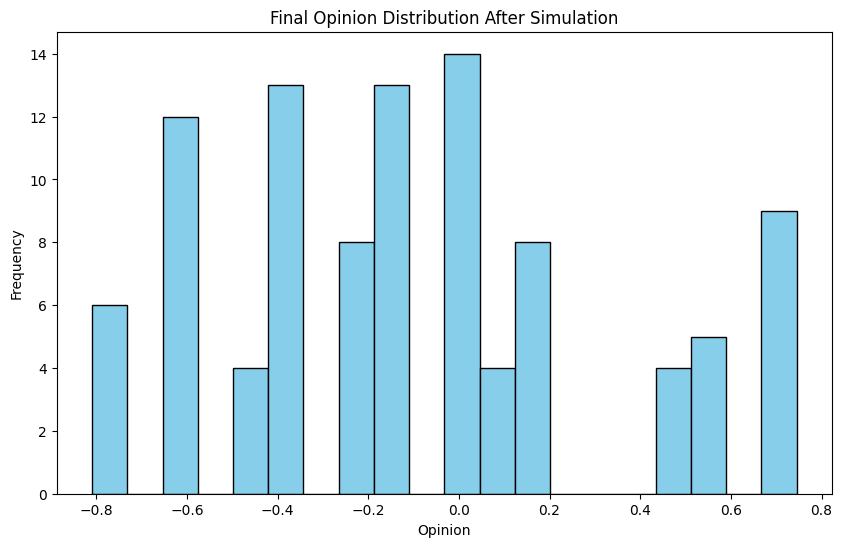
\includegraphics[width=0.6\linewidth]{download-11.png}
    \caption{Final distribution of nodes in the network at stationary state}
    \label{fig:finopinion}
\end{figure}

\subsection{Opinion Variance}
Opinion variance measures the spread of opinions within the network. The Y-axis represents variance of values of opinions at each time step represented by X-axis. The initial decline indicates that agents are rapidly aligning their opinions with those of their neighbors, which reduces the overall spread of opinions.

After around 40-50 time steps, the variance levels off and remains relatively constant at a low value. This plateau indicates that the opinion dynamics have reached a steady state, where further opinion adjustments are minimal, and agents have largely formed stable opinion clusters.(Figure \ref{fig:opiniondist}).

\begin{figure}[h]
    \centering
    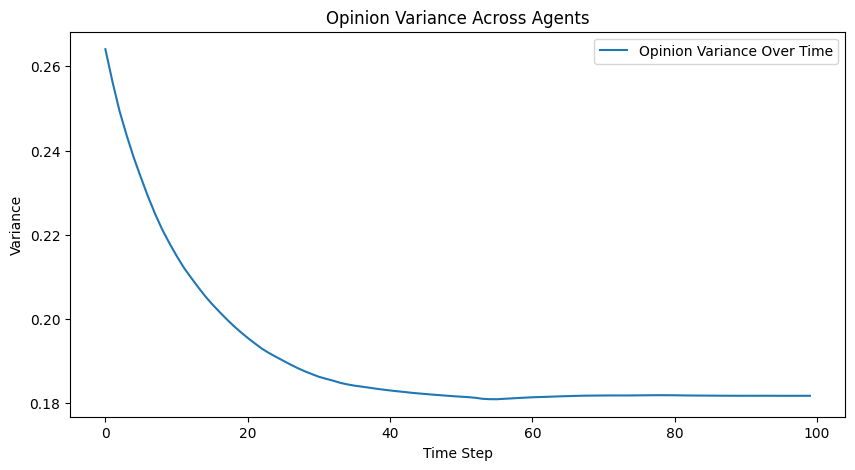
\includegraphics[width=0.8\linewidth]{download-7.png}
    \caption{Opinion Variance distribution w.r.t. Time}
    \label{fig:opiniondist}
\end{figure}

\subsection{Diversity Index (Entropy) Over Time}
Calculated using entropy, this index captures the overall diversity of opinions. Similar to the Opinion Variance, we found that the higher entropy suggested higher variation in opinions and following with a rapid decline indicates that agents are quickly adjusting their opinions and clustering with similar neighbors, reducing the diversity in opinions. (Figure \ref{fig:opiniondiversity}).

\begin{figure}[h]
    \centering
    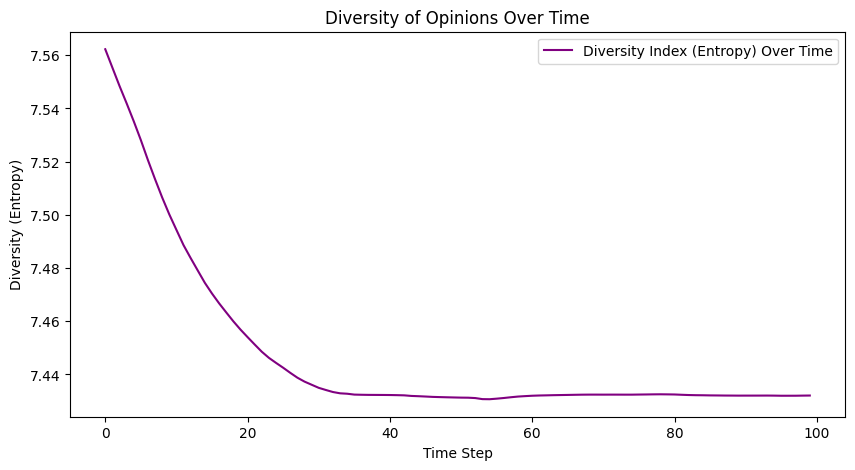
\includegraphics[width=0.8\linewidth]{download-8.png}
    \label{fig:opiniondiversity}
\end{figure}


\subsection{Rewiring Events Over Time}
This plot represents how frequently agents in the network change their connections based on opinion similarity.

The number of rewiring events varies significantly over time, with no clear trend of continuous increase or decrease. This fluctuation suggests that rewiring is responsive to the dynamic changes in agents' opinions and connections rather than following a linear pattern. This suggests that network has not fully stabilized after the initial cluster formation and is actively participating in the re-evaluation of connections (Figure \ref{fig:clusterdist}).

\begin{figure}[h]
    \centering
    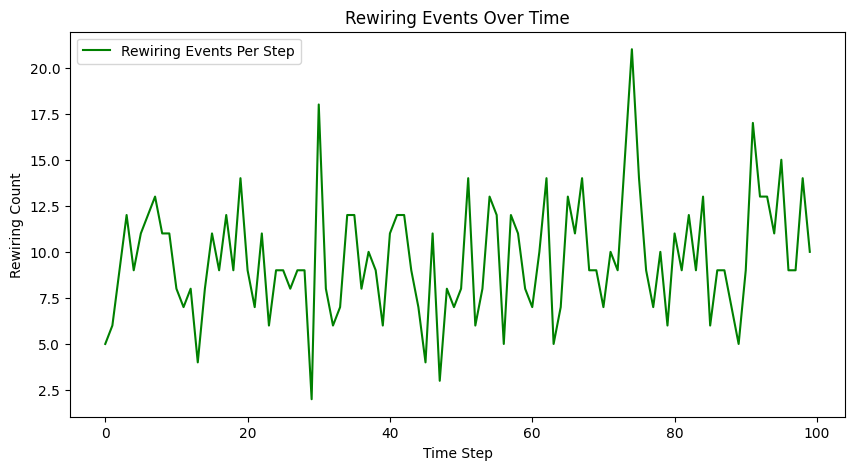
\includegraphics[width=0.8\linewidth]{download-9.png}
    \label{fig:clusterdist}
\end{figure}

\section{Conclusion}

\begin{table}[t]
\caption{Values of initial parameters taken}
\label{sample-table}
\begin{center}
\begin{tabular}{ll}
\multicolumn{1}{c}{\bf PARAMETERS}  &\multicolumn{1}{c}{\bf VALUE}
\\ \hline \\
No. of Agents          &100 \\
No. of Initial Links             &300 \\
Homophily Factor             &0.5 \\
Steps             &100 \\
\end{tabular}
\end{center}
\end{table}

This study explores the formation of echo chambers in social networks through a homophily-based model of opinion dynamics. By simulating agents who update their opinions and rewire connections based on similarity, we observe the powerful influence of homophily in clustering individuals with like-minded peers, causing emergence of distinct opinion groups.

The results show how homophily-driven rewiring of the network induces strong initial speedup of opinion convergence in the formation of clusters, stable groups where agents mainly interact with agents with similar opinions. This effect is evident in the decreasing opinion variance and entropy, which reach steady states as agents settle into echo chambers. However, the sustained level of rewiring activity suggests that while the network reaches a relatively stable configuration, it remains slightly fluid, with minor reconfigurations occurring over time due to boundary agents or small opinion shifts.

The study underscores the effectiveness of homophily in driving network polarization, showing how social networks can naturally fragment into echo chambers even without external influence. The presence of multiple opinion clusters suggests a realistic balance of diversity within echo chambers, mirroring real-world social dynamics where subgroups maintain distinct viewpoints within broader communities.

Overall, this research contributes to our understanding of echo chamber formation by providing a model that captures the nuanced effects of homophily and opinion alignment. Future work could further investigate the impact of varying homophily factors, network size, and influence strengths to gain deeper insights into the mechanisms that underlie polarization in complex social systems. This understanding is crucial for developing strategies to address polarization in online platforms, where echo chambers can limit exposure to diverse perspectives and exacerbate social divides.


\bibliographystyle{abbrv}
\bibliography{references}

\end{document}
